\documentclass[tikz,border=4pt]{standalone}
\usepackage[T1]{fontenc}
\usepackage{mathptmx}
\usetikzlibrary{arrows.meta,calc}
\begin{document}
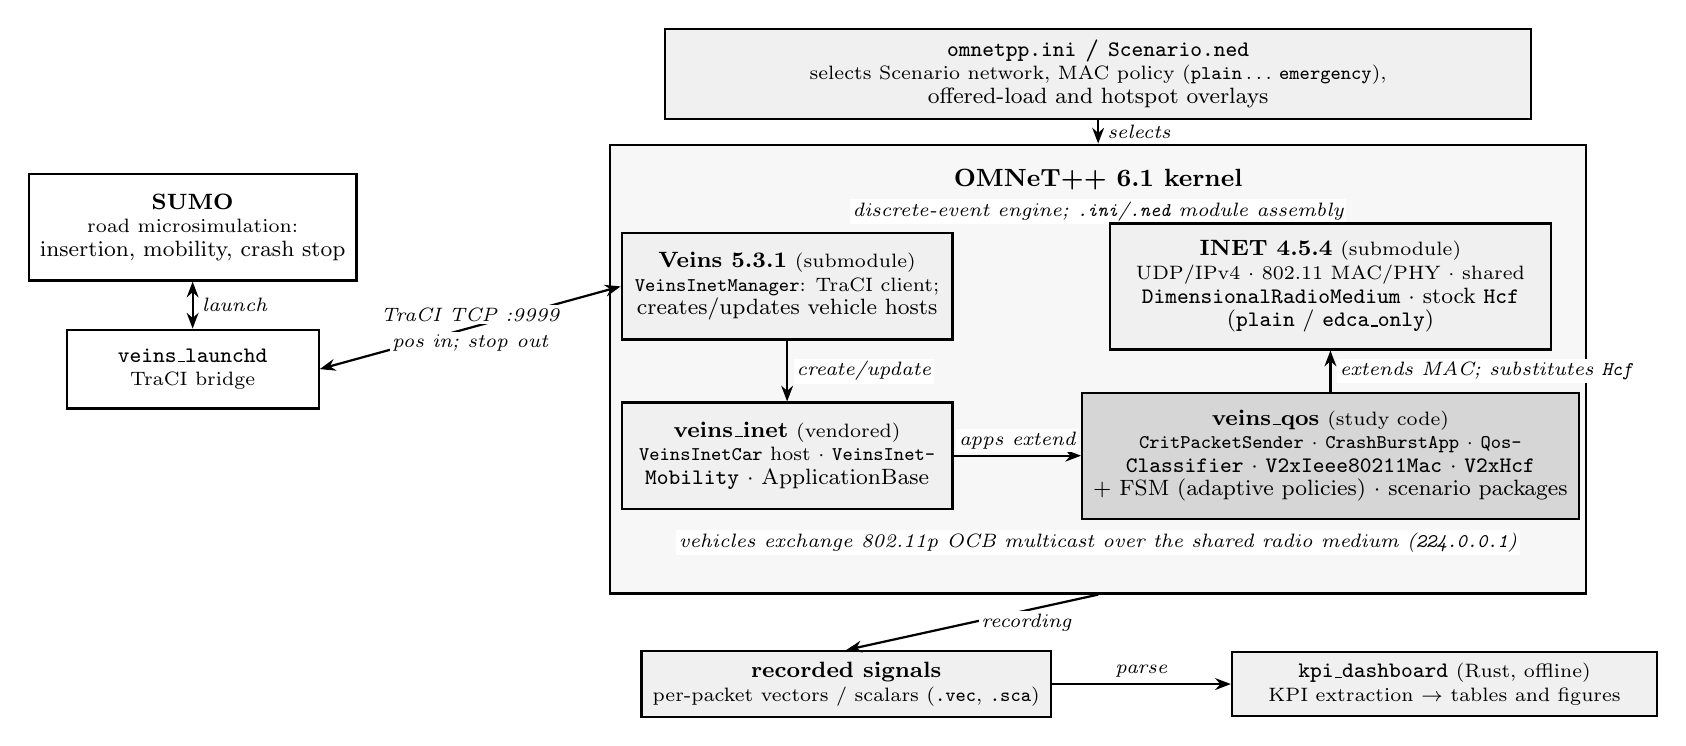
\begin{tikzpicture}[
  font=\footnotesize,
  >=Stealth,
  thick,
  box/.style={draw, thick, align=center, inner sep=4pt},
  ext/.style={box, fill=white},
  fw/.style={box, fill=black!6},
  study/.style={box, fill=black!16},
  kernel/.style={box, fill=black!3, inner sep=8pt},
  arr/.style={-{Stealth[length=2.0mm]}, thick},
  biarr/.style={{Stealth[length=2.0mm]}-{Stealth[length=2.0mm]}, thick},
  lab/.style={font=\scriptsize\itshape, align=center, fill=white, inner sep=1pt},
  ktitle/.style={font=\small\bfseries},
]

  % ===== Configuration (top) =====
  \node[fw, minimum width=11.0cm] (conf) at (8.8,8.9)
    {\textbf{\texttt{omnetpp.ini} / \texttt{Scenario.ned}}\\[-1pt]
     \scriptsize selects Scenario network, MAC policy (\texttt{plain}\,\dots\,\texttt{emergency}),\\[-1pt]
     offered-load and hotspot overlays};

  % ===== External road simulator (left) =====
  \node[ext, minimum width=3.2cm, minimum height=1.35cm] (sumo) at (-2.7,6.95)
    {\textbf{SUMO}\\[-1pt]
     \scriptsize road microsimulation:\\[-1pt]
     insertion, mobility, crash stop};
  \node[ext, minimum width=3.2cm, minimum height=1.0cm] (launchd) at (-2.7,5.15)
    {\texttt{veins\_launchd}\\[-1pt]
     \scriptsize TraCI bridge};
  \draw[biarr] (sumo) -- (launchd);
  \node[lab, right=2pt] at ($(sumo.south)!0.5!(launchd.north)$) {launch};

  % ===== OMNeT++ kernel container =====
  \node[kernel, minimum width=12.4cm, minimum height=5.7cm] (kern) at (8.8,5.15) {};
  \node[ktitle] at (8.8,7.55) {OMNeT++ 6.1 kernel};
  \node[lab] at (8.8,7.15) {discrete-event engine; \texttt{.ini}/\texttt{.ned} module assembly};

  \node[fw, minimum width=4.2cm, minimum height=1.35cm] (veins) at (4.85,6.2)
    {\textbf{Veins 5.3.1} \scriptsize(submodule)\\[-1pt]
     \scriptsize \texttt{VeinsInetManager}: TraCI client;\\[-1pt]
     creates/updates vehicle hosts};
  \node[fw, minimum width=4.2cm, minimum height=1.35cm] (vend) at (4.85,4.05)
    {\textbf{veins\_inet} \scriptsize(vendored)\\[-1pt]
     \scriptsize \texttt{VeinsInetCar} host $\cdot$ \texttt{VeinsInet-}\\[-1pt]
     \texttt{Mobility} $\cdot$ ApplicationBase};
  \node[fw, minimum width=5.6cm, minimum height=1.6cm] (inet) at (11.75,6.2)
    {\textbf{INET 4.5.4} \scriptsize(submodule)\\[-1pt]
     \scriptsize UDP/IPv4 $\cdot$ 802.11 MAC/PHY $\cdot$ shared\\[-1pt]
     \texttt{DimensionalRadioMedium} $\cdot$ stock \texttt{Hcf}\\[-1pt]
     (\texttt{plain} / \texttt{edca\_only})};
  \node[study, minimum width=5.6cm, minimum height=1.6cm] (qos) at (11.75,4.05)
    {\textbf{veins\_qos} \scriptsize(study code)\\[-1pt]
     \scriptsize \texttt{CritPacketSender} $\cdot$ \texttt{CrashBurstApp} $\cdot$ \texttt{Qos-}\\[-1pt]
     \texttt{Classifier} $\cdot$ \texttt{V2xIeee80211Mac} $\cdot$ \texttt{V2xHcf}\\[-1pt]
     + FSM (adaptive policies) $\cdot$ scenario packages};

  % ===== Arrows inside/around the kernel =====
  \draw[biarr] (launchd.east) -- (veins.west)
    node[lab, midway, above=1pt] {TraCI TCP :9999}
    node[lab, midway, below=1pt] {pos in; stop out};
  \draw[arr] (veins) -- (vend) node[lab, midway, right=2pt] {create/update};
  \draw[arr] (qos) -- (inet) node[lab, midway, right=2pt] {extends MAC; substitutes \texttt{Hcf}};
  \draw[arr] (vend.east) -- (qos.west) node[lab, midway, above=1pt] {apps extend};
  \node[lab] at (8.8,2.95) {vehicles exchange 802.11p OCB multicast over the shared radio medium (\texttt{224.0.0.1})};

  \draw[arr] (conf.south) -- (kern.north) node[lab, midway, right=2pt] {selects};

  % ===== Offline analysis (bottom) =====
  \node[fw, minimum width=4.8cm] (rec) at (5.6,1.15)
    {\textbf{recorded signals}\\[-1pt]
     \scriptsize per-packet vectors / scalars (\texttt{.vec}, \texttt{.sca})};
  \node[fw, minimum width=5.4cm] (kpi) at (13.2,1.15)
    {\textbf{\texttt{kpi\_dashboard}} \scriptsize(Rust, offline)\\[-1pt]
     \scriptsize KPI extraction $\rightarrow$ tables and figures};
  \draw[arr] (kern.south) -- (rec.north) node[lab, midway, right=2pt] {recording};
  \draw[arr] (rec) -- (kpi) node[lab, midway, above=1pt] {parse};
\end{tikzpicture}
\end{document}
